

\documentclass[20pt,a3paper, landscape]{tikzposter}
\usepackage[utf8]{inputenc}
\usepackage{xcolor}
\usepackage{graphicx,mwe}

\usepackage{lipsum}
\usepackage{tikz}
\usepackage{multicol}
\usepackage{adjustbox}
\usepackage{blindtext}
\usepackage{comment}


 \makeatletter
\def\TP@titlegraphictotitledistance{-6cm}
\settitle{ \centering \vbox{
		\@titlegraphic \\ [\TP@titlegraphictotitledistance] 
		\centering
		\color{titlefgcolor} 
		{\bfseries \Huge \sc \@title \par}
		\vspace*{1em}
		{\huge \@author \par}
}}
\makeatother

\setlength{\columnsep}{2cm}
 
\title{Magic Faucet Fountain}
\author{Gruppe 07 - Asena Yüce, Carl-Lewis Maschke, Nina Braams, Sven Neumann, Valeria Kornichenkova} %\author{<Author>}
\titlegraphic{
\includegraphics[height=4cm]{images/logo_hs_technik}
	\hfill

\includegraphics[height=4cm]{images/logo}
}
 
 
\usetheme{Desert}
\colorlet{blocktitlebgcolor}{cyan!30!blue}
\setlength{\columnsep}{2cm}
 
\begin{document}
\maketitle


\begin{columns} 
	
	\column{0.5}
	{

		\block{Grundkonstruktion}
		{
			Der Magic Faucet Fountain ist ein innovatives Dekorationselemen, das durch eine clevere Konstruktion den Eindruck erweckt, ein Wasserhahn würde frei in der Luft schweben. 
			Der Effekt wird durch ein transparentes Acrylrohr erzeugt, das vom Wasserfluss verdeckt wird.
%			\begin{tikzfigure}
%				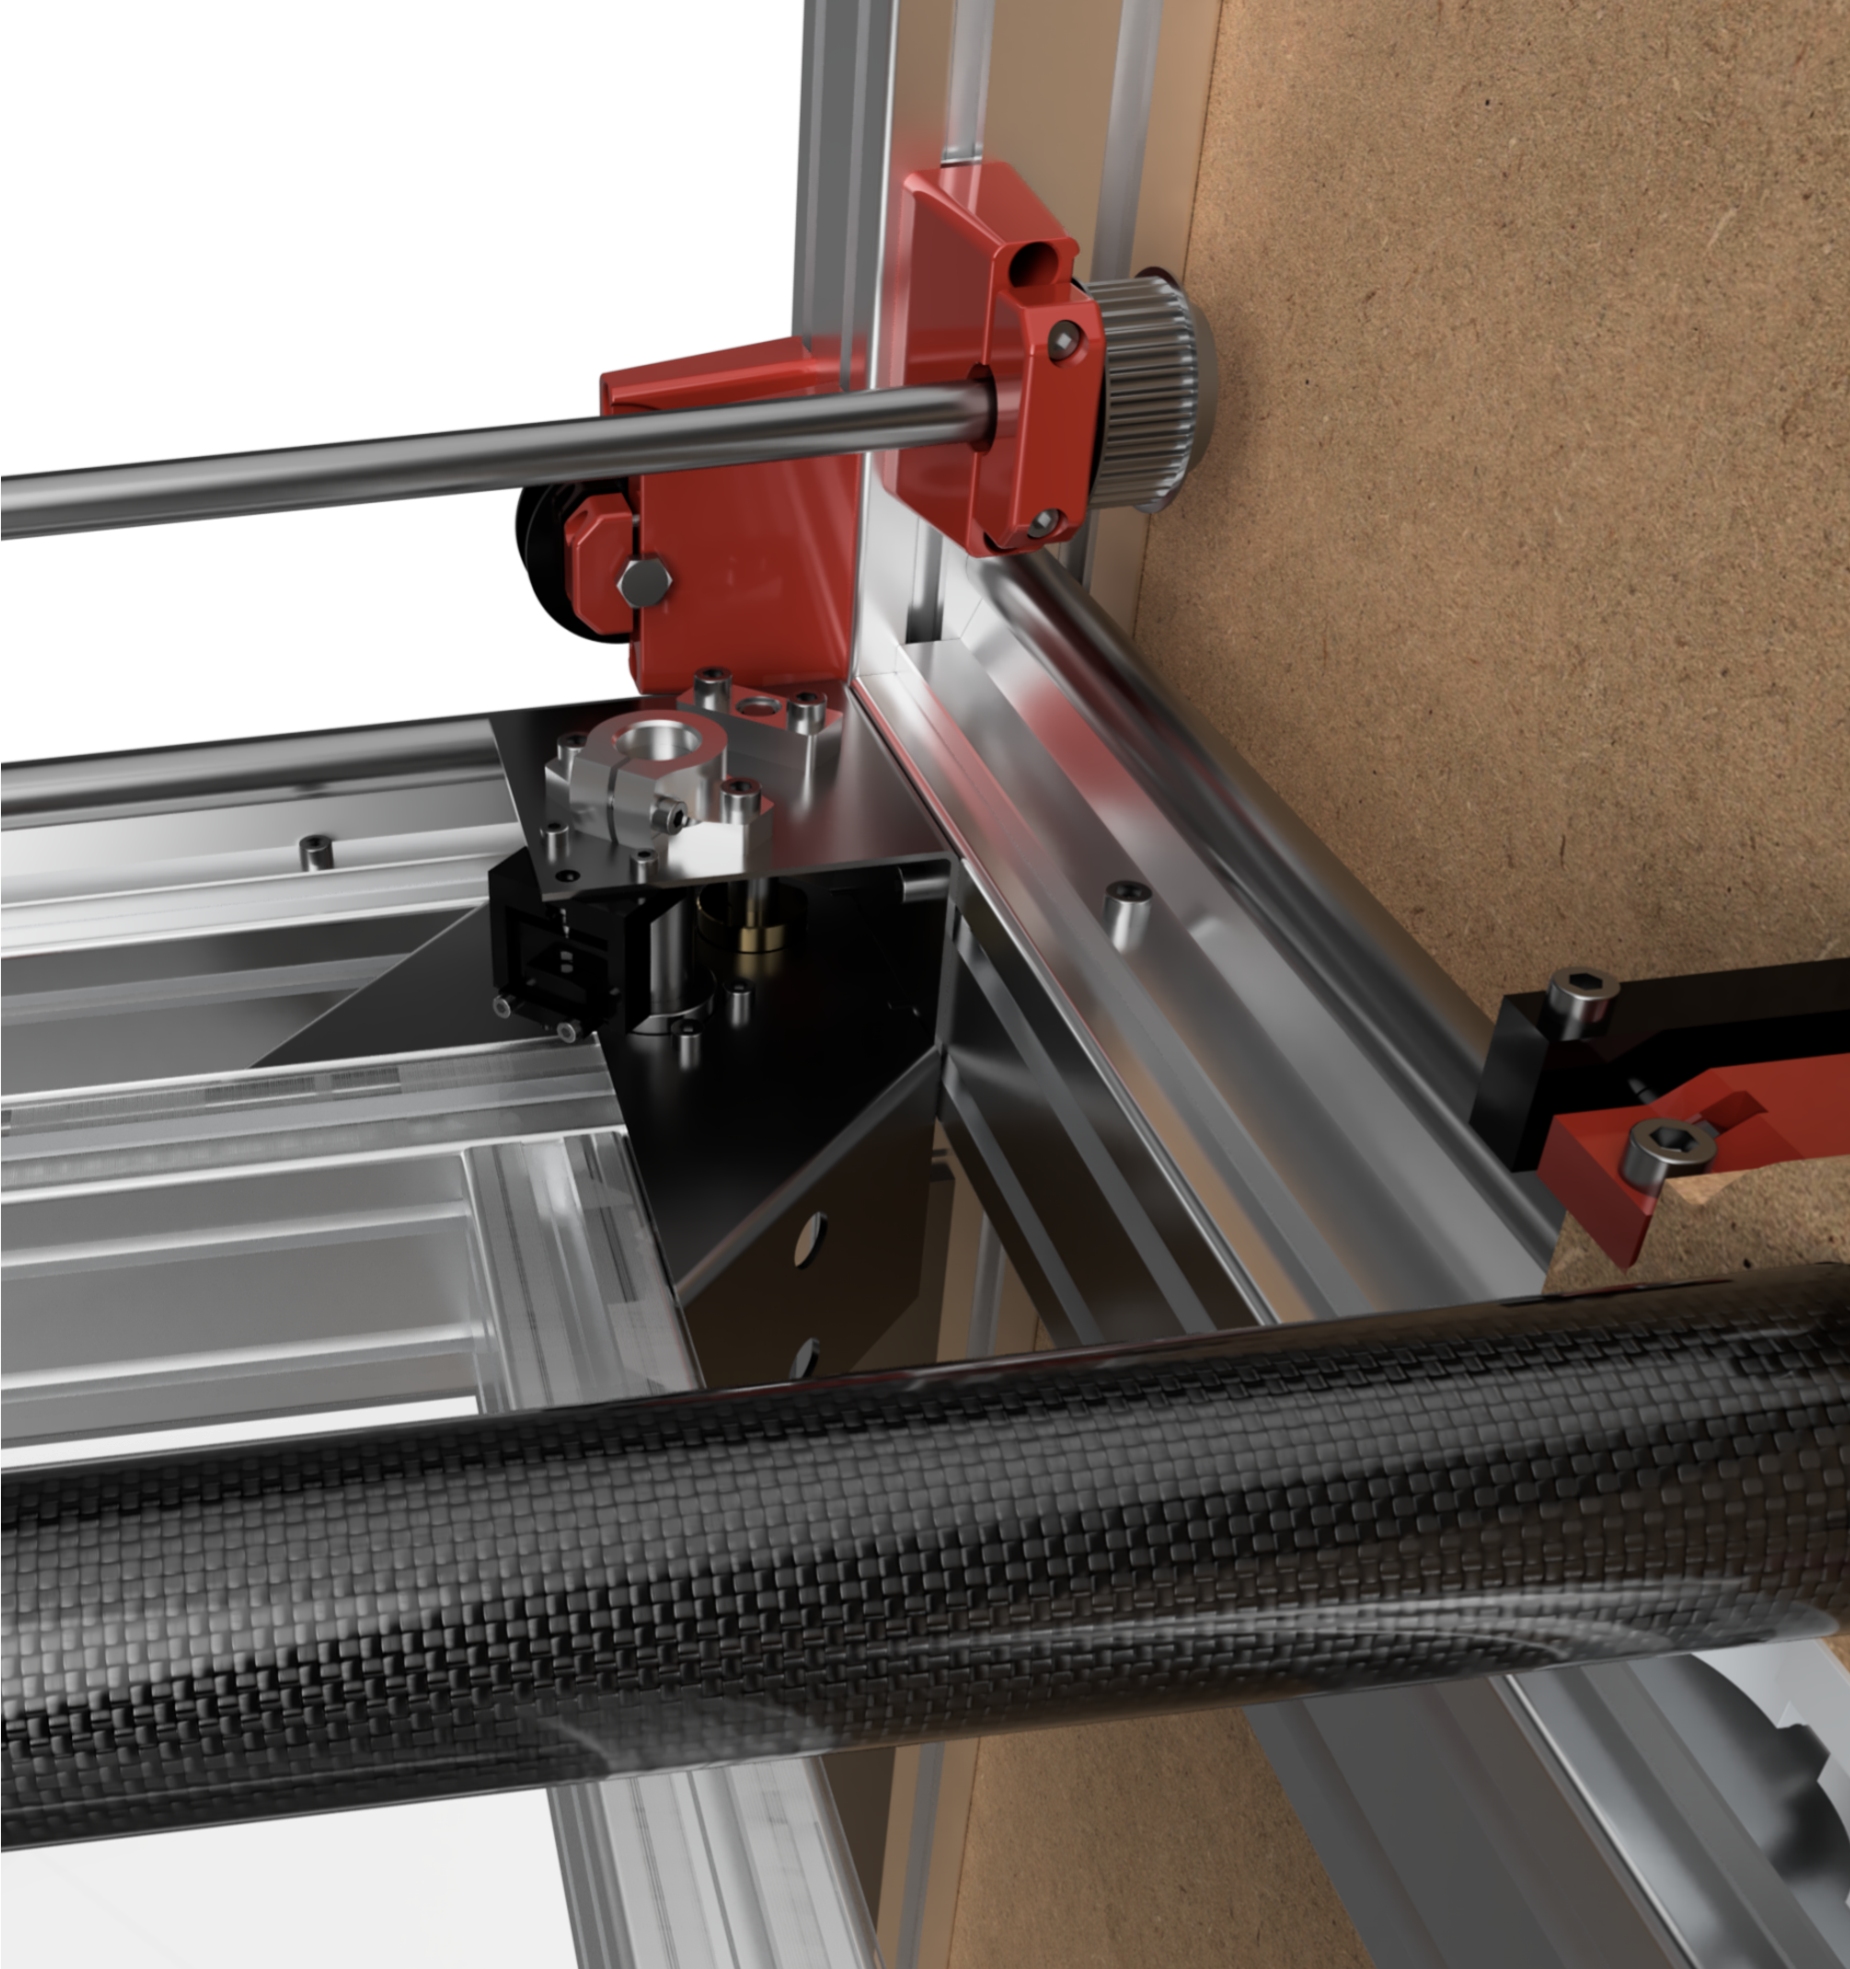
\includegraphics[width=\linewidth]{images/Rendering10}
%			\end{tikzfigure}	
		
		}
		\block{Digital Twin}
		{
			"The Digital Twin is a set of virtual information constructs that fully describes a potential or actual physical manufactured product from the micro atomic level to the macro geometrical level. At its optimum, any information that could be obtained from inspecting a physical manufactured product can be obtained from its Digital Twin."- Grieves \& Vickers (2016)
			
			Dabei besteht das Konzept Digital Twin aus drei wesentlichen Teilen, auf der einen Seite dem physischen Objekt in der Realen Welt, auf der anderen Seite dem digitalen Abbild in der virtuellen Welt und dazwischen liegt ein Datenaustausch zwischen diesen Instanzen vor. So fließen kontinuierlich Daten vom realen Objekt an das virtuelle um dieses zu präzisieren und umgekehrt helfen die Daten aus den Simulationen das reale Objekt besser zu verstehen.
		}
		\block{Herausforderungen}
		{
			\begin{itemize}
				\item Konstruktion eines unsichtbaren Trägers für den Wasserhahn
				\item Integration eines Sensors zur Pegelmessung im engen Raum
				\item Stromversorgung bei gleichzeitiger Wassersicherheit
				\item App-Anbindung via Bluetooth mit Arduino Nano 33 BLE Sense
			\end{itemize}
		}
		
		\block{Lösungen}
		{
			\begin{itemize}
				\item Acrylrohr mit passendem Durchmesser und transparenter Optik
				\item Schwimmer + Ultraschallsensor für präzise Pegelkontrolle
				\item Abgesicherter Netzteilkasten mit Hauptschalter
				\item RemoteXY-App zur Steuerung via Bluetooth
			\end{itemize}
		}
		\block{Ergebnisse}
		{
			Der Fountain funktioniert zuverlässig. Die App-Anbindung wurde erfolgreich getestet. 
			Die Wasserstandsmessung ermöglicht automatische Warnungen bei niedrigem Pegel. 
			Die Bauweise ist einfach zu warten und modular.
		}
		
	}


	\column{0.5}
	{
		\colorlet{blocktitlebgcolor}{blue}
		\block{Rendering}
		{
			\begin{tikzfigure}
				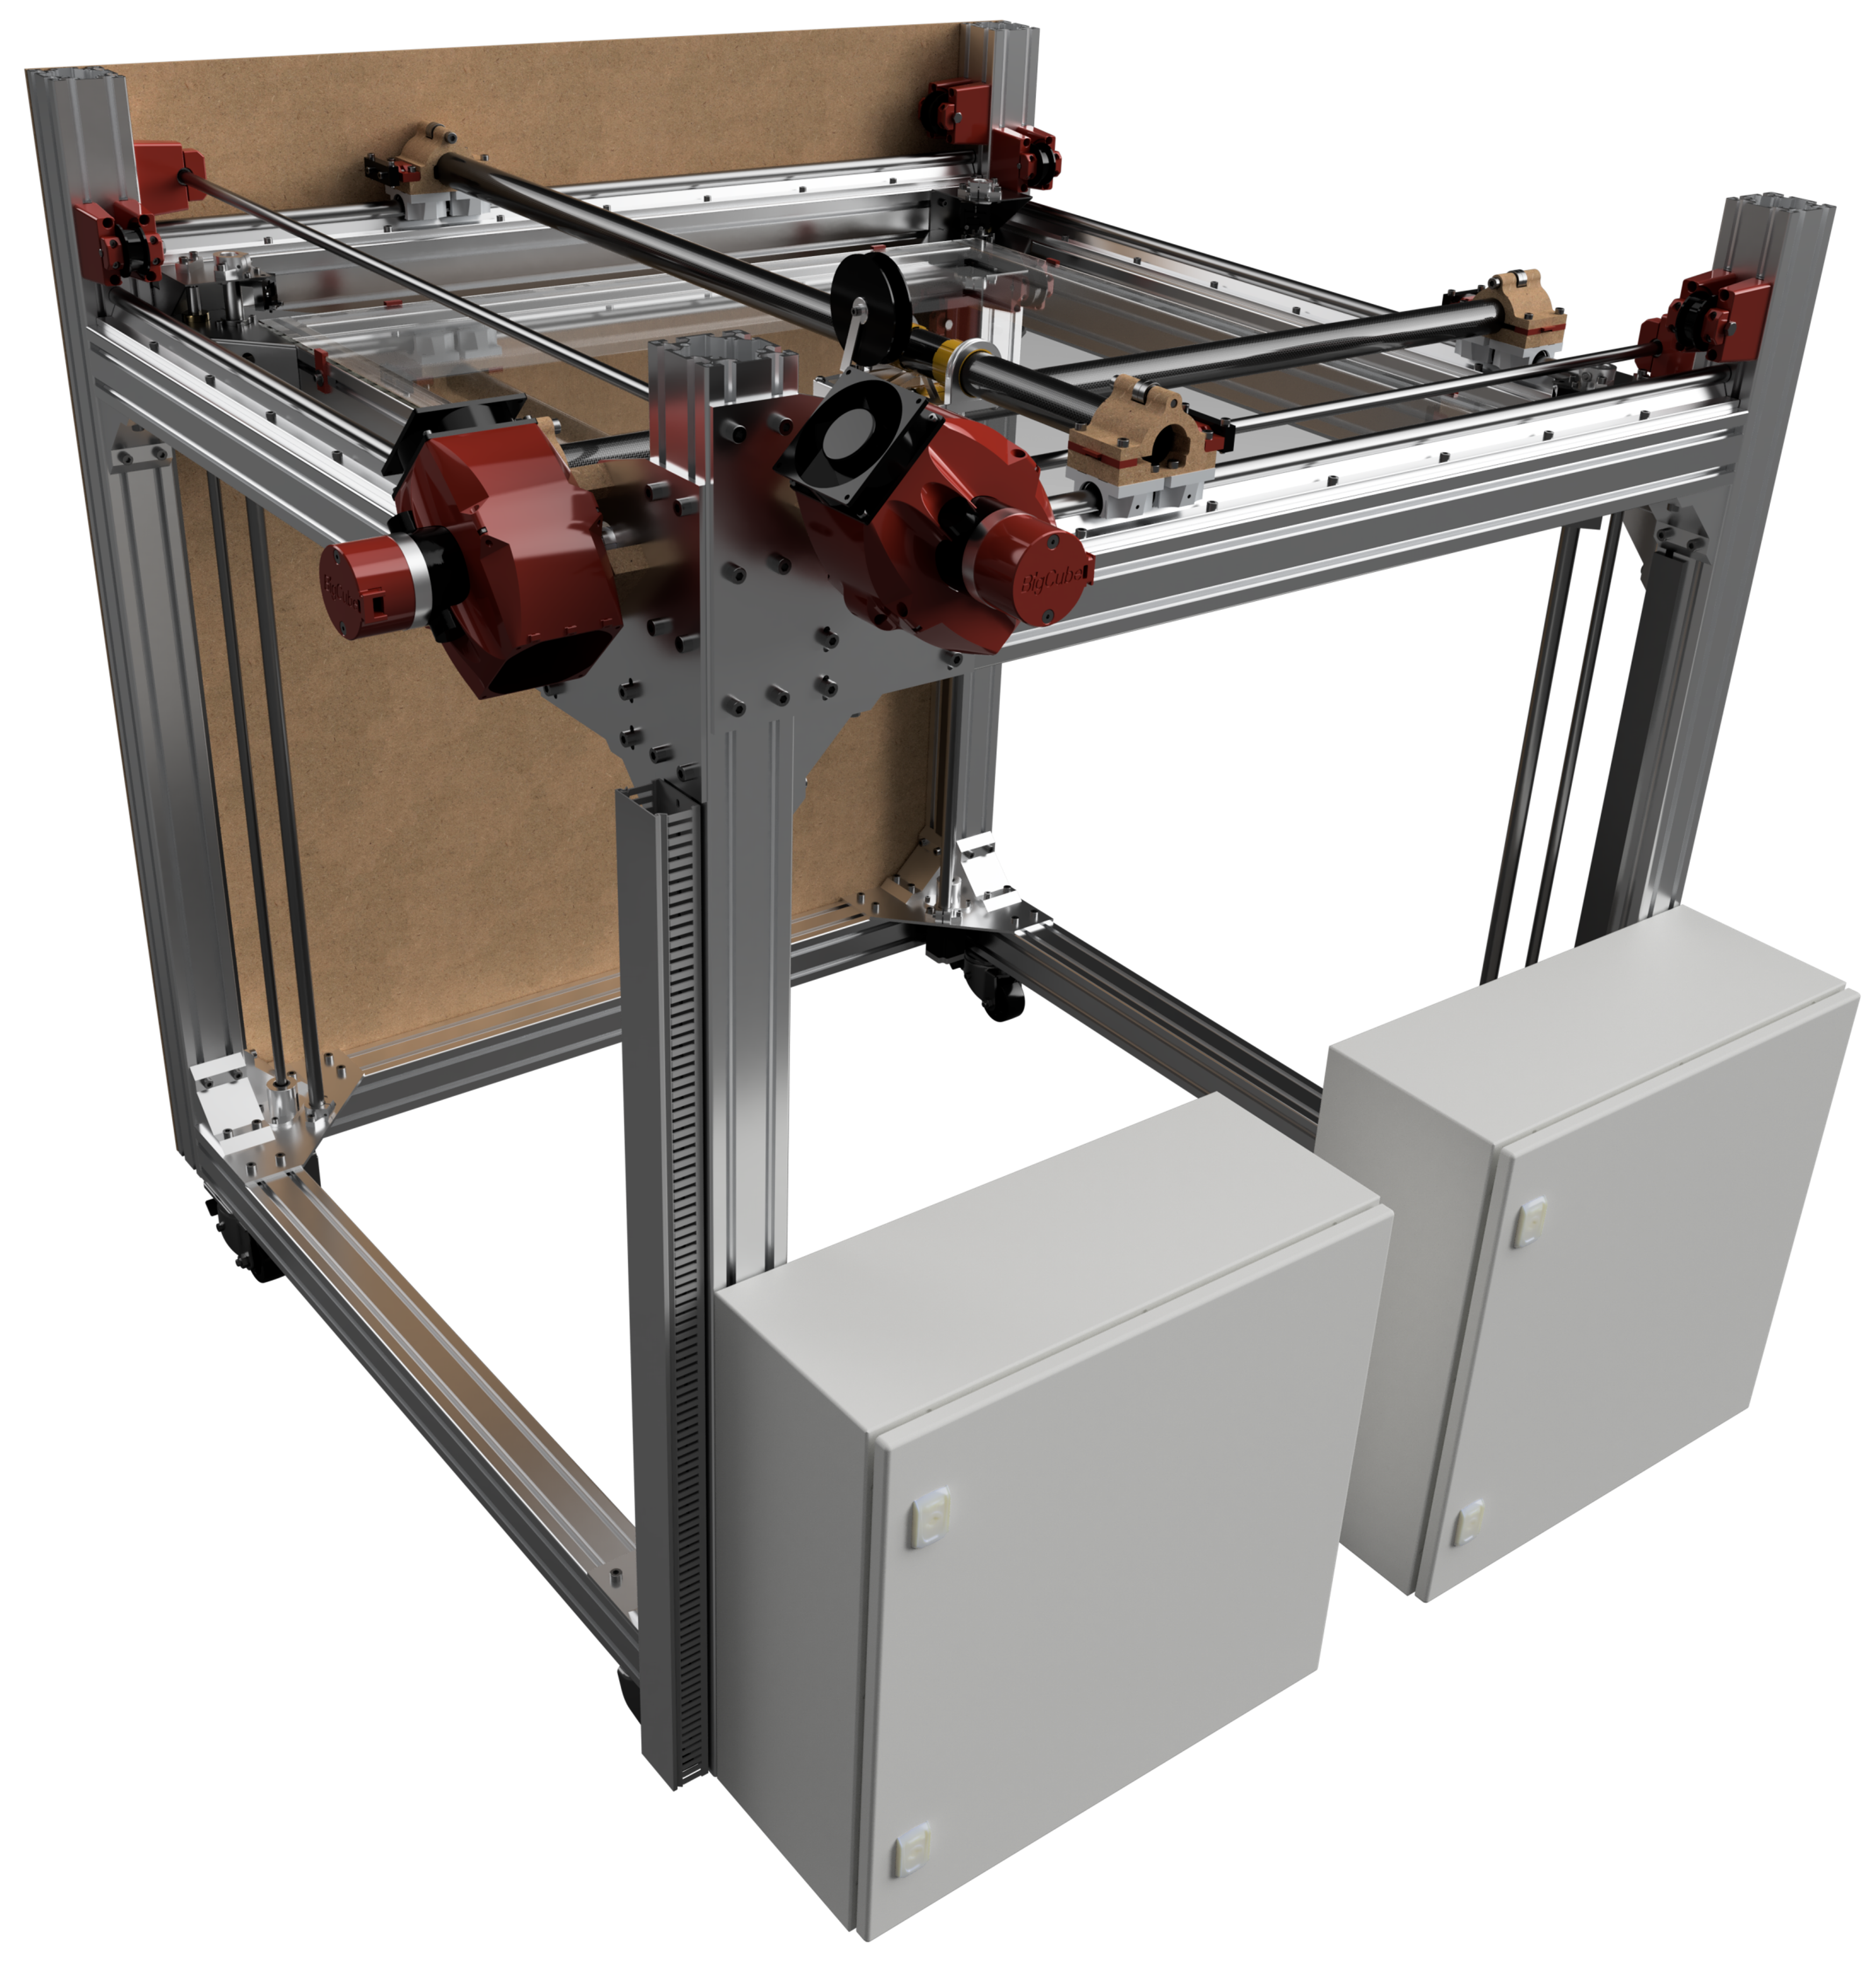
\includegraphics[width=\linewidth]{images/Rendering9}
			\end{tikzfigure}
		}
	}
\end{columns}

\begin{columns} 
	
	\column{0.5}
	{
		\colorlet{blocktitlebgcolor}{blue}
		\block{Rendering Draufsicht}
		{
			\begin{tikzfigure}
				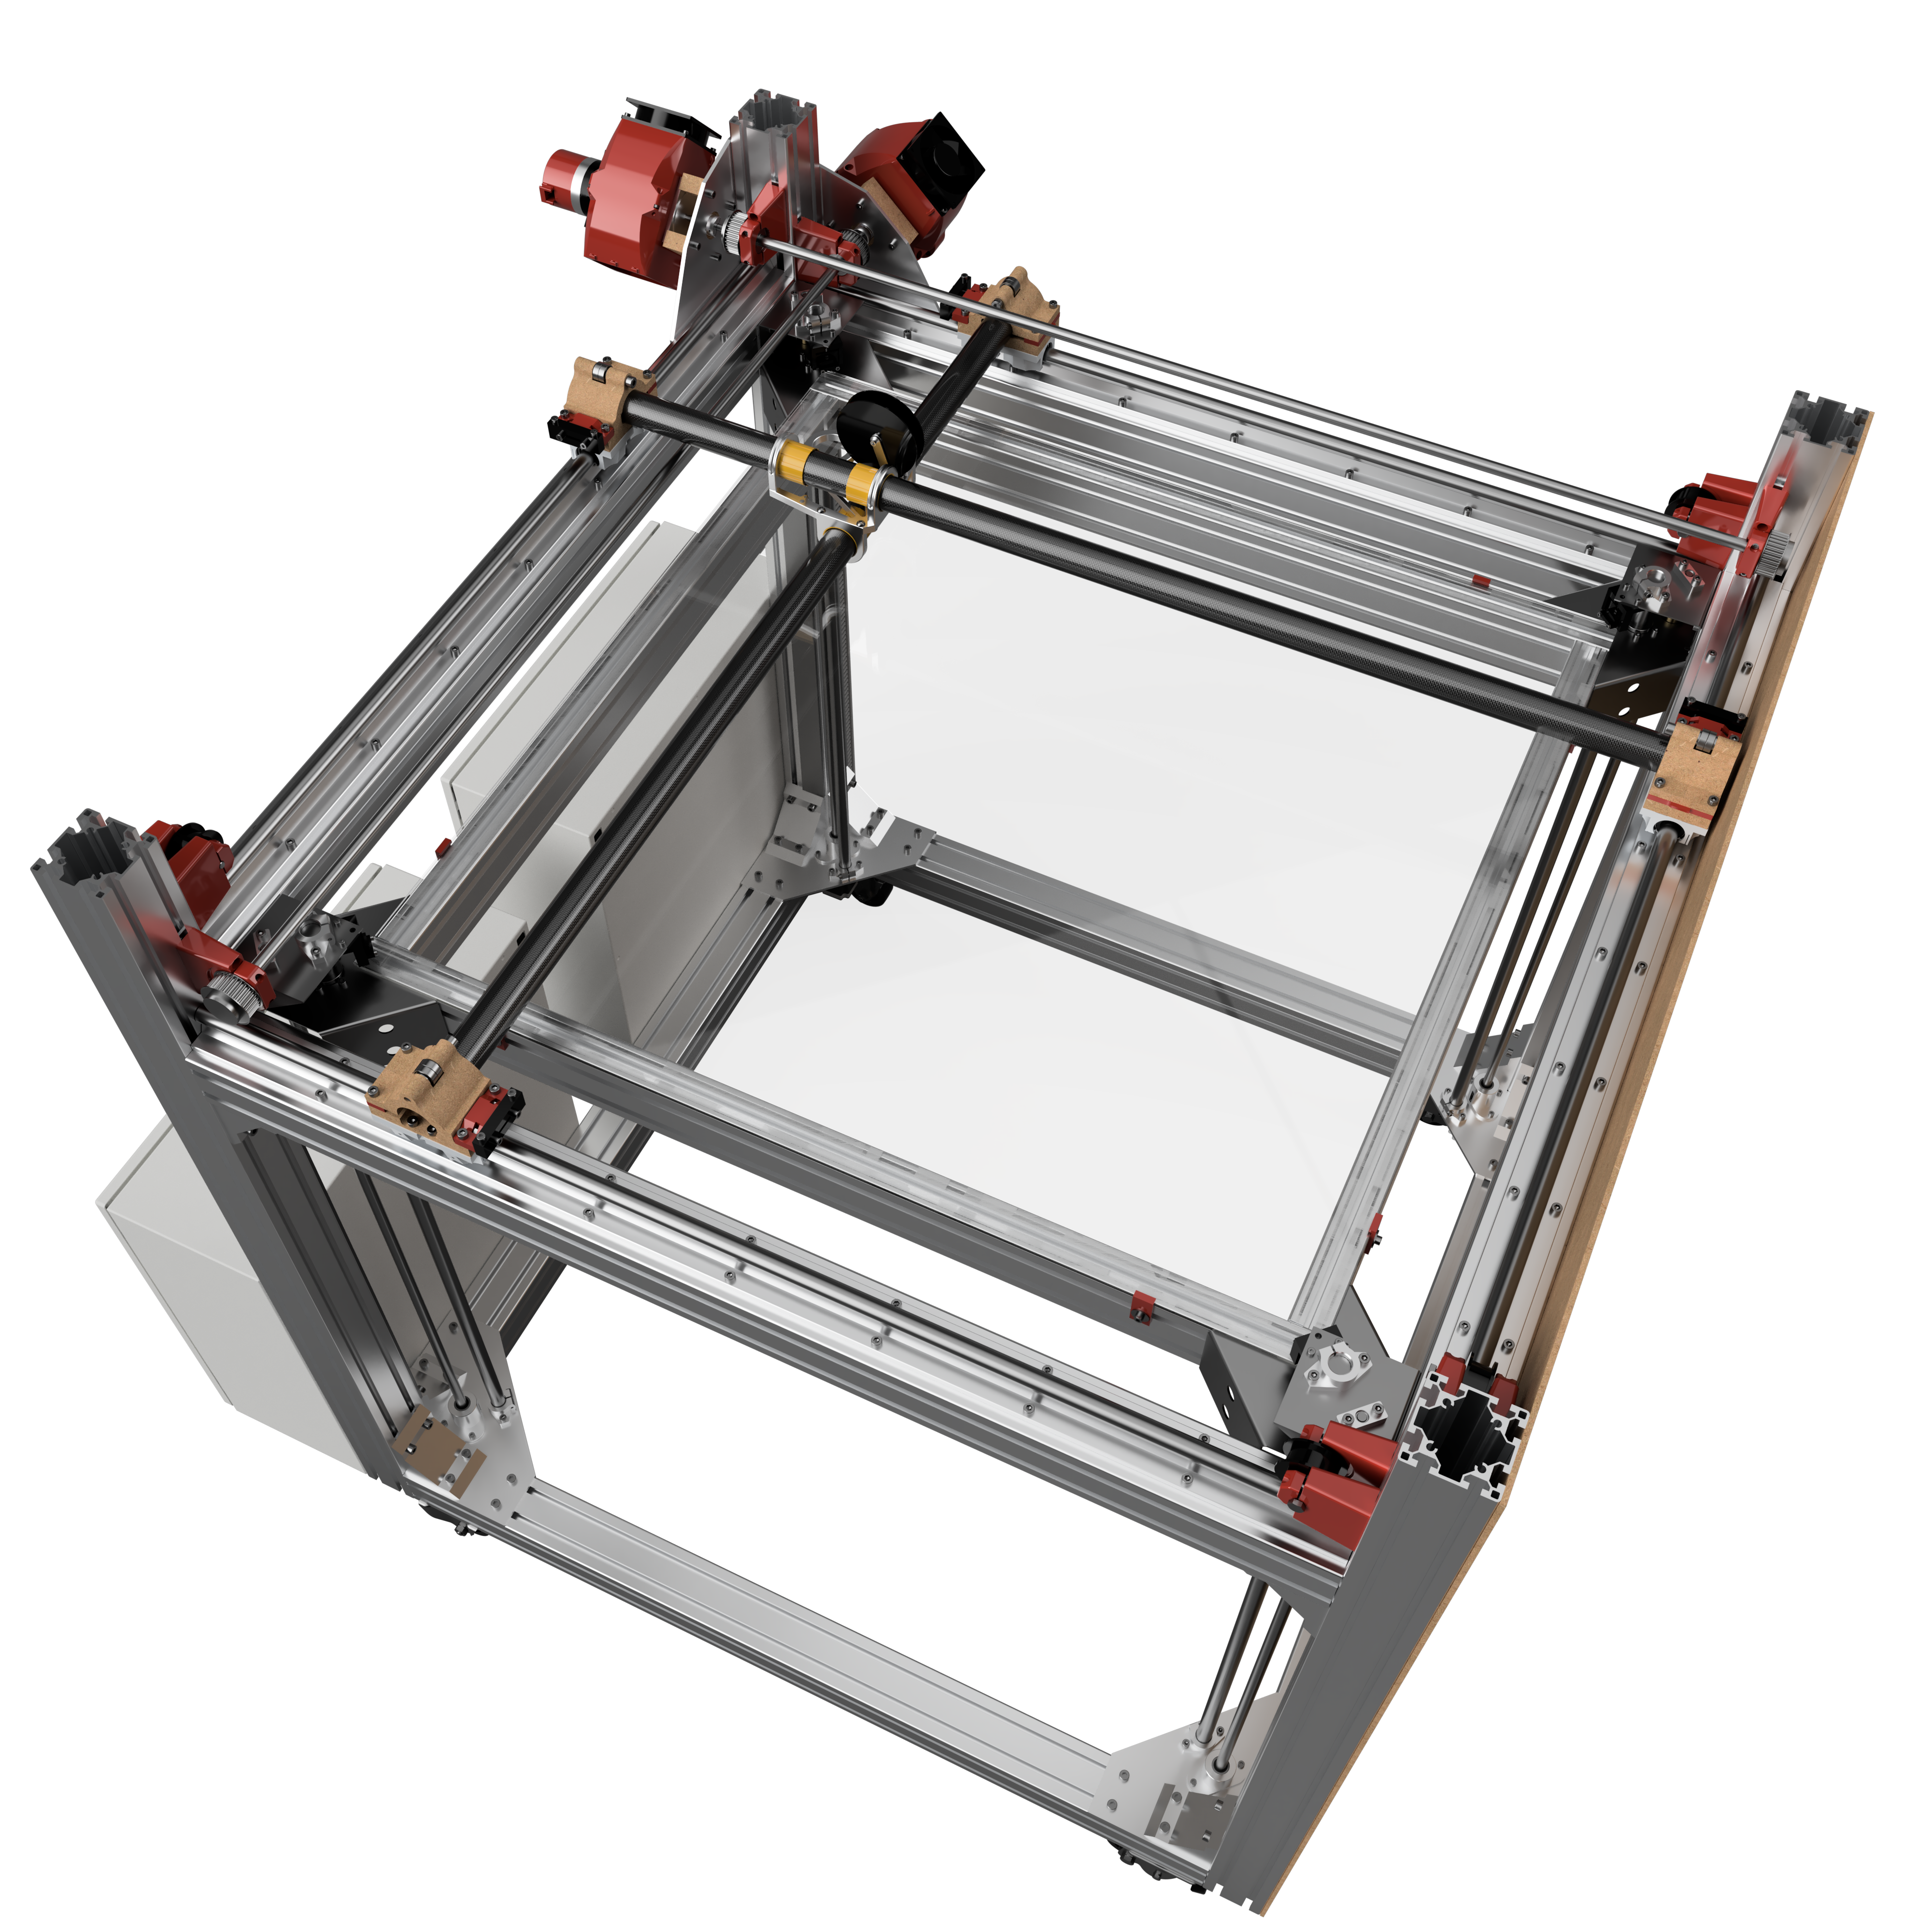
\includegraphics[width=\linewidth]{images/Rendering8}
			\end{tikzfigure}	
		}
	}
	
	
	\column{0.5}
	{
		\colorlet{blocktitlebgcolor}{blue}
	\block{Funktionsskizze in TikZ}
	{
		\begin{center}
			\begin{tikzpicture}[scale=0.8]
				% Blumentopf
				\draw[thick] (0,0) ellipse (2 and 0.5);
				\draw[thick] (-2,0) -- (-2,2.5) arc[start angle=180,end angle=360,radius=2cm and 0.5cm] -- (2,0);
				\draw[dashed] (0,0.5) ellipse (1 and 0.25);
				
				% Acrylrohr
				\draw[thick] (0,2.5) -- (0,6);
				\draw[blue, thick] (0,6) -- (0,7);
				\node at (0.7,6.5) {Wasser};
				
				% Wasserhahn
				\draw[thick] (0,7) -- (0.5,7);
				\draw[thick] (0.5,7) -- (0.5,6.8);
				\draw[thick] (0.5,6.8) -- (0.3,6.8);
				
				% Fallendes Wasser
				\draw[blue, thick] (0.3,6.8) -- (0.3,5.5);
				
				% Beschriftungen
				\node at (0,-1) {Blumentopf};
				\node at (-1.2,3.5) {Acrylrohr};
				\node at (1.5,7) {Wasserhahn};
			\end{tikzpicture}
		\end{center}
	}
	
	\block{App-GUI mit TikZ}
	{
		\begin{center}
			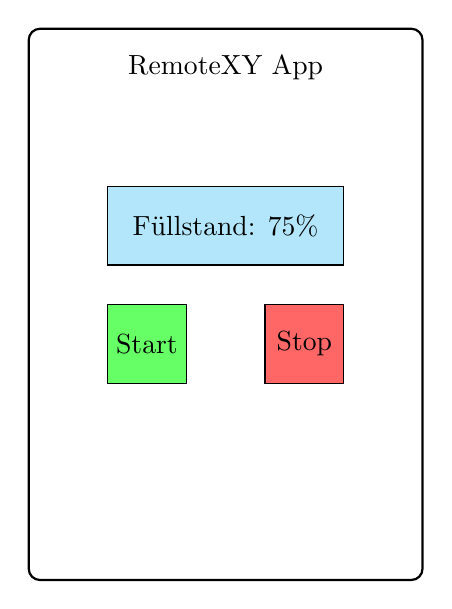
\begin{tikzpicture}
				% App Rahmen
				\draw[rounded corners, thick] (0,0) rectangle (5,7);
				\node at (2.5,6.5) {RemoteXY App};
				% Anzeige Wasserstand
				\draw[fill=cyan!30] (1,4) rectangle (4,5);
				\node at (2.5,4.5) {F\"ullstand: 75\%};
				% Buttons
				\draw[fill=green!60] (1,2.5) rectangle (2,3.5);
				\draw[fill=red!60] (3,2.5) rectangle (4,3.5);
				\node at (1.5,3) {Start};
				\node at (3.5,3) {Stop};
			\end{tikzpicture}
		\end{center}
	}
	\end{columns}

\end{document}

